\documentclass[11pt]{article}
\usepackage{amssymb}
\usepackage{amsthm}
\usepackage{enumitem}
\usepackage{physics,amsmath}
\usepackage{bm}
\usepackage{adjustbox}
\usepackage{mathrsfs}
\usepackage{graphicx}
\usepackage{siunitx}
\usepackage[mathscr]{euscript}

\title{\textbf{Solved selected problems of Classical Mechanics - Gregory}}
\author{Franco Zacco}
\date{}

\addtolength{\topmargin}{-3cm}
\addtolength{\textheight}{3cm}

\newcommand{\hatr}{\bm{\hat{r}}}
\newcommand{\hatx}{\bm{\hat{x}}}
\newcommand{\haty}{\bm{\hat{y}}}
\newcommand{\hatz}{\bm{\hat{z}}}
\newcommand{\hatn}{\bm{\hat{n}}}
\newcommand{\hati}{\bm{\hat{i}}}
\newcommand{\hatj}{\bm{\hat{j}}}
\newcommand{\hatk}{\bm{\hat{k}}}
\newcommand{\uvi}{\bm{i}}
\newcommand{\uvj}{\bm{j}}
\newcommand{\uvk}{\bm{k}}
\newcommand{\hatth}{\bm{\hat{\theta}}}
\newcommand{\hatphi}{\bm{\hat{\phi}}}
\newcommand{\hatrho}{\bm{\hat{\rho}}}
\newcommand{\ngrad}[1]{\text{grad}_{\bm{#1}}}

\theoremstyle{definition}
\newtheorem*{solution*}{Solution}
\renewcommand*{\proofname}{\bf{Solution}}

\begin{document}
\maketitle
\thispagestyle{empty}

\section*{Chapter 18 - Tensor algebra and the inertia tensor}

\begin{proof}{\textbf{18.3}}
    Let the matrix $\bm{A}$ be
    \begin{align*}
        \bm{A} = \frac{1}{3}\begin{pmatrix}
            2 & -1 & -2\\
            2 & 2  & 1\\
            1 & -2 & 2
        \end{pmatrix}
    \end{align*}
    If $\bm{A}$ is orthogonal it must happen that
    $\bm{A}\cdot \bm{A}^T = \bm{1}$ then we see that
    \begin{align*}
        \frac{1}{9}\begin{pmatrix}
            2 & -1 & -2\\
            2 & 2  & 1\\
            1 & -2 & 2
        \end{pmatrix} \cdot
        \begin{pmatrix}
            2 & 2 & 1\\
            -1 & 2  & -2\\
            -2 & 1 & 2
        \end{pmatrix}
        &= \frac{1}{9}\begin{pmatrix}
            4 + 1 + 4 & 4 - 2 - 2 & 2 + 2 - 4\\
            4 - 2 - 2 & 4 + 4 + 1 & 2 - 4 + 2\\
            2 + 2 - 4 & 2 - 4 + 2 & 1 + 4 + 4
        \end{pmatrix}\\
        &= \frac{1}{9}\begin{pmatrix}
            9 & 0 & 0\\
            0 & 9 & 0\\
            0 & 0 & 9
        \end{pmatrix}\\
        &= \begin{pmatrix}
            1 & 0 & 0\\
            0 & 1 & 0\\
            0 & 0 & 1
        \end{pmatrix} = \bm{1}
    \end{align*}
    Therefore $\bm{A}$ is orthogonal.\\
    Now we check $\bm{A}$ has determinant +1 as follows
    \begin{align*}
        \frac{1}{3^3}\det\begin{pmatrix}
            2 & -1 & -2\\
            2 & 2  & 1\\
            1 & -2 & 2
        \end{pmatrix} &= \frac{1}{27}[(8 -1 + 8) - (-4 -4 -4)]\\
        &= \frac{1}{27}[15 + 12]\\
        &= 1
    \end{align*}
    Next, we want to find the column vector $\bm{v}$ that satisfies the equation
    $\bm{A}\cdot\bm{v} = \bm{v}$ so if we assume that $\bm{v} = (v_1, v_2, v_3)$
    by solving the matrix multiplication we get that
    \begin{align*}
        v_1 = \frac{2}{3}v_1 - \frac{1}{3}v_2 - \frac{2}{3}v_3\\
        v_2 = \frac{2}{3}v_1 + \frac{2}{3}v_2 + \frac{1}{3}v_3\\
        v_3 = \frac{1}{3}v_1 - \frac{2}{3}v_2 + \frac{2}{3}v_3
    \end{align*}
    Hence by subtracting the second equation to the first equation we get that
    \begin{align*}
        v_1 - v_2 &= -v_2 - v_3\\
        v_1 &= -v_3
    \end{align*}
    Now we replace the value of $v_1$ in the third equation to get 
    \begin{align*}
        v_3 &= -\frac{1}{3}v_3 - \frac{2}{3}v_2 + \frac{2}{3}v_3\\
        v_3 - \frac{1}{3}v_3 &= - \frac{2}{3}v_2\\
        v_3 &= -v_2
    \end{align*}
    Therefore we see that $v_2 = v_1$ and $v_3 = -v_1$ so the column vector
    that satisfies this equation is
    \begin{align*}
        \bm{v} = v_1\begin{pmatrix}
            1\\ 1\\ -1
        \end{pmatrix}
    \end{align*}
    Where $v_1$ can take any value.

    Given that $\det(\bm{A}) = +1$ we know that $\bm{A}$ represents a rotation
    about some axis passing through $O$ but we see that the vector
    $\bm{v} = (1, 1, -1)$ is not changed when multiplied by $\bm{A}$ so the
    vector $\bm{v}$ has exactly the same coordinates in the system $C'$, this
    implies that $\bm{v}$ must lay in the axis of rotation, therefore $\bm{A}$
    represents a rotation about an axis passing through $E = (1, 1, -1)$.

    Finally, since $\bm{A}$ is a rotation matrix about an axis with unit vector
    $\bm{n} = (1/\sqrt{3}, 1/\sqrt{3}, -1/\sqrt{3})$ it must happen that $\bm{A}$
    is of the form of the equation (18.10) so we can use this equation
    to determine the rotation angle as follows
    \begin{align*}
        &\begin{pmatrix}
            \cos\psi + (1-\cos\psi)n_1^2 & (1-\cos\psi)n_1n_2 + n_3\sin\psi & (1-\cos\psi)n_1n_3 - n_2\sin\psi\\
            (1-\cos\psi)n_2n_1 - n_3\sin\psi & \cos\psi + (1-\cos\psi)n_2^2  & (1-\cos\psi)n_2n_3 + n_1\sin\psi\\
            (1-\cos\psi)n_3n_1 + n_2\sin\psi & (1-\cos\psi)n_3n_2 - n_1\sin\psi & \cos\psi + (1-\cos\psi)n_3^2
        \end{pmatrix}\\
        &=\begin{pmatrix}
            \cos\psi + (1-\cos\psi)/3 &
            (1-\cos\psi)/3 -\sin\psi/\sqrt{3} &
            -(1-\cos\psi)/3 - \sin\psi/\sqrt{3}\\
            (1-\cos\psi)/3 + \sin\psi/\sqrt{3} &
            \cos\psi + (1-\cos\psi)/3 &
             -(1-\cos\psi)/3 + \sin\psi/\sqrt{3}\\
            -(1-\cos\psi)/3 + \sin\psi/\sqrt{3} &
            -(1-\cos\psi)/3 - \sin\psi/\sqrt{3} &
            \cos\psi + (1-\cos\psi)/3
        \end{pmatrix}\\
        &=\begin{pmatrix}
            2\cos\psi/3 + 1/3 &
            1/3-\cos\psi/3 -\sin\psi/\sqrt{3} &
            -1/3+\cos\psi/3 - \sin\psi/\sqrt{3}\\
            1/3-\cos\psi/3 + \sin\psi/\sqrt{3} &
            2\cos\psi/3 + 1/3 &
             -1/3 +\cos\psi/3 + \sin\psi/\sqrt{3}\\
            -1/3 +\cos\psi/3 + \sin\psi/\sqrt{3} &
            -1/3+\cos\psi/3 - \sin\psi/\sqrt{3} &
            2\cos\psi/3 + 1/3
        \end{pmatrix}
    \end{align*}
    Taking the element in the first row and column and making it equal to the
    value we have from $\bm{A}$ we get that $2\cos(\psi)/3 + 1/3 = 2/3$ then
    $\cos\psi= 1/2$ therefore the angle of rotation must be $\psi = \pi/3$.
\end{proof}
\cleardoublepage
\begin{proof}{\textbf{18.7}}
    Let $\{v_i\}$ be a first order tensor, and let us also consider the outer
    product $\{v_iv_j\}$ then we know that the trace of this second order
    tensor is invariant but the trace of $\{v_iv_j\}$ is $v_1^2 + v_2^2 +v_3^2$
    therefore the sum of the squares of the elements of $\{v_i\}$ is invariant.

    Let $\{t_{ij}\}$ be a second order tensor then the outer product
    $\{t_{ij}t_{nm}\}$ is a fourth order tensor and hence the trace of this
    tensor is 
    \begin{align*}
        \sum_{i=1}^3\sum_{j=1}^3 t_{ij}t_{ij}
    \end{align*}
    which we know is invariant. Therefore the sum of the squares of the
    elements of $\{t_{ij}\}$ is invariant.
\end{proof}
\begin{proof}{\textbf{18.8}}
    Let $\bm{T}$ be a second order tensor. We want to show that $\det \bm{T}$
    is an invariant. We know that $\bm{T}$ transforms to a different coordinate
    system as
    \begin{align*}
        \bm{T'} = \bm{A \cdot T\cdot A^{T}}
    \end{align*}
    Then
    \begin{align*}
        \det (\bm{T'}) &= \det (\bm{A \cdot T\cdot A^{T}})\\
            &= \det (\bm{A})\det(\bm{T})\det(\bm A^{T})\\
            &= \pm 1\cdot\det(\bm{T})\cdot \pm 1\\
            &= \det(\bm{T})
    \end{align*}
    Where we used that $\det (\bm{A}) = \det (\bm{A}^T)$ is $\pm 1$.
    Therefore the determinant of $\bm{T}$ will have the value $\det\bm{T}$ in
    any coordinate system, hence it's an invariant.
\end{proof}
\cleardoublepage
\begin{proof}{\textbf{18.10}}
    Let us consider the following rigid body
    \begin{center}
        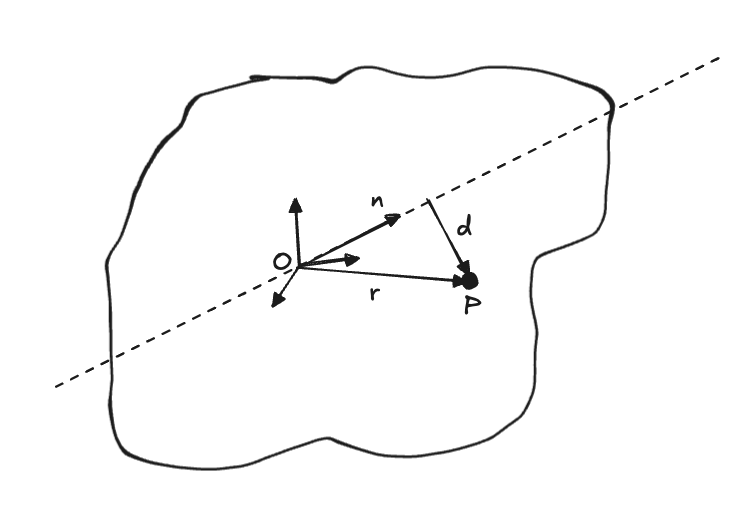
\includegraphics[scale=0.35]{ch18-10.png}
    \end{center}
    Where $\bm n$ is the unit vector, $P$ is the i-th particle of the rigid body
    and $\bm{r}$ is the distance from O to the particle. Then the distance
    $d$ is
    \begin{align*}
        d^2 &= \bm{r}\cdot\bm{r} - (\bm{n\cdot r})^2
    \end{align*} 
    Where we used that $\bm{n\cdot r}$ is the component of $\bm{r}$ on the line
    described by $\bm{n}$. Then by using the components of each vector
    we have that
    \begin{align*}
        d^2 &= (r_1^2 + r_2^2 + r_3^2) - (n_1r_1 + n_2r_2 + n_3r_3)^2\\
        &= (r_1^2 + r_2^2 + r_3^2) - (n_1^2r_1^2 + n_2^2r_2^2 + n_3^2r_3^2
        + 2n_1r_1n_2r_2 + 2n_1r_1n_3r_3 + 2n_2r_2n_3r_3)\\
        &= (1- n_1^2)r_1^2 + (1 - n_2^2)r_2^2 + (1 - n_3^2)r_3^2
        - 2n_1r_1n_2r_2 - 2n_1r_1n_3r_3 - 2n_2r_2n_3r_3\\
        &= (n_2^2 + n_3^2)r_1^2 + (n_1^2 + n_3^2)r_2^2 + (n_1^2 + n_2^2)r_3^2
        - 2n_1r_1n_2r_2 - 2n_1r_1n_3r_3 - 2n_2r_2n_3r_3\\
        &= (r_2^2 + r_3^2)n_1^2 + (r_1^2+ r_3^2)n_2^2 + (r_1^2 + r_2^2)n_3^2 
        - 2n_1r_1n_2r_2 - 2n_1r_1n_3r_3 - 2n_2r_2n_3r_3
    \end{align*}
    If we multiply the equation by the mass of each particle $P$ in the rigid
    body and we sum over all of them we get that
    \begin{align*}
        \sum md^2 &= \sum m(r_2^2 + r_3^2)n_1^2 + m(r_1^2+ r_3^2)n_2^2 +
        m(r_1^2 + r_2^2)n_3^2 \\
        &\quad - 2mn_1r_1n_2r_2 - 2mn_1r_1n_3r_3 - 2mn_2r_2n_3r_3
    \end{align*}
    So we see that $I_{\{O,\bm{n}\}} = \sum md^2$, the first three terms are
    the moments of inertia of each particle with respect to the axis $x_1$,
    $x_2$ and $x_3$ respectively and the rest are twice the negative products
    of inertia multiplied by two of the coordiantes of the unit vector
    so we can write this equation as
    \begin{align*}
        I_{\{O,\bm{n}\}} &= I_{11}n_1^2 + I_{22}n_2^2 + I_{33}n_3^2
        + 2I_{12}n_1n_2 + 2I_{13}n_1n_3 + 2I_{23}n_2n_3\\
        &= n_1(I_{11}n_1 + I_{12}n_2 + I_{13}n_3)
        + n_2(I_{22}n_2 + I_{12}n_1 + I_{23}n_3)\\
        &\quad+ n_3(I_{33}n_3 + 2I_{13}n_1 + I_{23}n_2)
    \end{align*}
    Which is the same as $I_{\{O,\bm{n}\}} = \bm{n^T \cdot I_O \cdot n}$.
\cleardoublepage
    Finally, let us consider a rectangular uniform plate of sides $2a$ and $2b$
    as shown below
    \begin{center}
        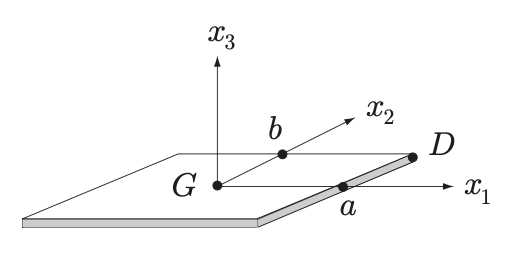
\includegraphics[scale=0.4]{ch18-10-2.png}
    \end{center}
    We know that the inertia tensor with respect to $G$ is
    \begin{align*}
        I_G = \frac{1}{3}M\begin{pmatrix}
            b^2 & 0 & 0\\
            0 & a^2 & 0\\
            0 & 0 & a^2 + b^2
        \end{pmatrix}
    \end{align*}
    We want to compute the moment of inertia about the diagonal described by 
    a unit vector with components $a/\sqrt{a^2 + b^2}$ and $b/\sqrt{a^2 + b^2}$
    then by applying the previous result we have that
    \begin{align*}
        I_{G, \bm{n}} =
        \bigg(\frac{a}{\sqrt{a^2 + b^2}}, \frac{b}{\sqrt{a^2 + b^2}}, 0\bigg)
        \cdot \frac{1}{3}M\begin{pmatrix}
            b^2 & 0 & 0\\
            0 & a^2 & 0\\
            0 & 0 & a^2 + b^2
        \end{pmatrix}
        \cdot \begin{pmatrix}
            \frac{a}{\sqrt{a^2 + b^2}}\\ \frac{b}{\sqrt{a^2 + b^2}}\\ 0
        \end{pmatrix}
    \end{align*}
    Therefore
    \begin{align*}
        I_{\{G, \bm{n}\}} &= \frac{1}{3}M\bigg(
        \frac{a^2}{a^2 + b^2}b^2 + \frac{b^2}{a^2 + b^2}a^2
        \bigg)\\
        I_{\{G, \bm{n}\}} &= \frac{2M}{3} \frac{a^2b^2}{a^2 + b^2}
    \end{align*}
\end{proof}
\cleardoublepage
\begin{proof}{\textbf{18.11}}
\begin{itemize}
    \item [(i)] Let us consider a uniform circular disk of mass $M$ and radius
    $a$ and a coordinate system as shown below on the centre of mass $G$ of the 
    disk
    \begin{center}
        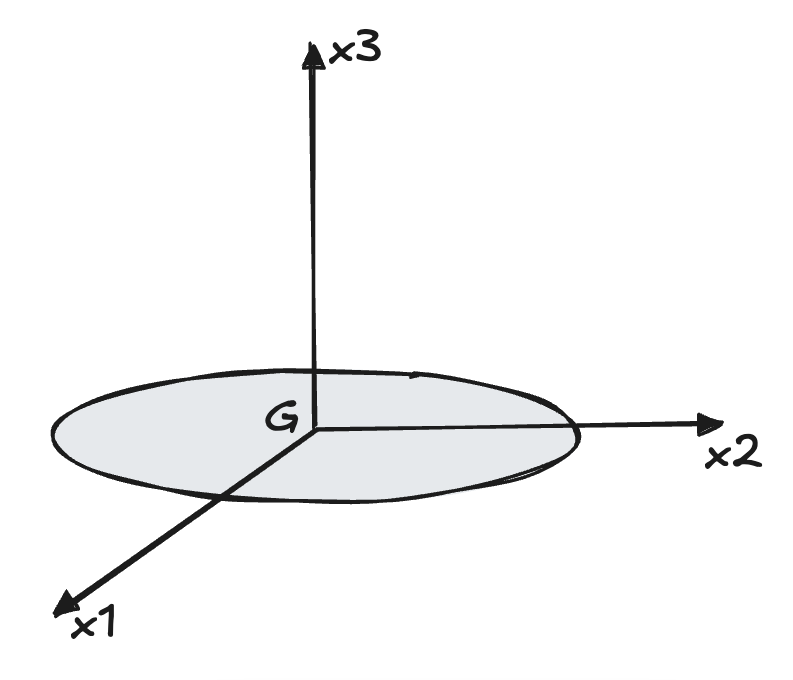
\includegraphics[scale=0.25]{ch18-11-i.png}
    \end{center}
    Around the axis $Gx_3$ the disk has rotational symmetry and around the axes
    $Gx_1$ and $Gx_2$ the disk has reflective symmetry so they are principal 
    axes of inertia, which implies that the principal moments of inertia
    with respect to these axes are
    \begin{align*}
        A &= \frac{1}{4}Ma^2\\
        B &= \frac{1}{4}Ma^2\\
        C &= \frac{1}{2}Ma^2
    \end{align*}
    \item [(ii)] Let us consider now the same uniform circular disk of mass $M$
    and radius $a$ and a coordinate system as shown below at a point $C$ on the
    edge of the disk
    \begin{center}
        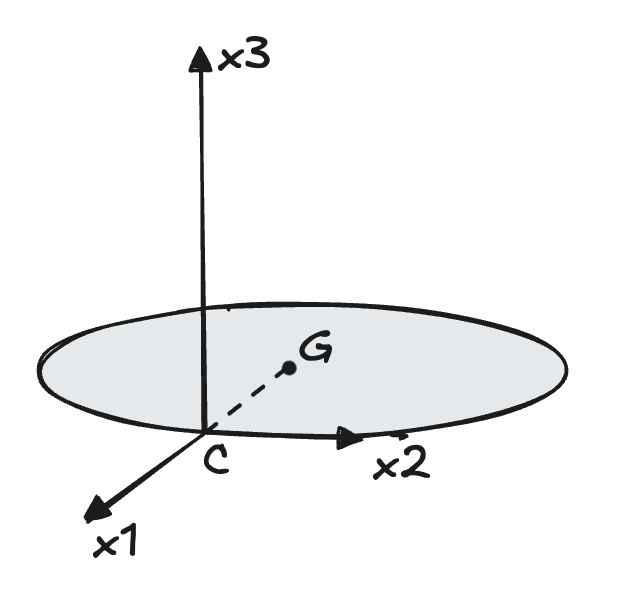
\includegraphics[scale=0.25]{ch18-11-ii.png}
    \end{center}
    Around the axis $Cx_1$ the disk has reflective symmetry and around the
    planes $x_2 = 0$ and $x_3 = 0$ the disk has reflective symmetry so they are
    principal axes of inertia, which implies that the principal moments of
    inertia with respect to these axes are
    \begin{align*}
        A &= \frac{1}{4}Ma^2\\
        B &= \frac{1}{4}Ma^2 + Ma^2 = \frac{5}{4}Ma^2\\
        C &= \frac{1}{2}Ma^2 + Ma^2 = \frac{3}{2}Ma^2
    \end{align*}
    Where we used the parallel axis theorem to compute them.
    
\end{itemize}
\end{proof}
\cleardoublepage
\begin{proof}{\textbf{18.17}}
\begin{itemize}
    \item [(i)] A frisbee is dynamically axially symmetric because it has a
    rotational symmetry about the symmetry axis.
    \item [(ii)] A piece of window glass having the shape of an isosceles
    triangle has no dynamical symmetry because the axis where we have
    rotational symmetry is of order two.
    \item [(iii)] A two bladed aircraft propellor has no dynamical symmetry
    because it has two rotationally symmetric axes but both of them are of
    order two.
    \item [(iv)] A three bladed ship propellor is dynamically axially
    symmetric because it is rotationally symmetric of order three with respect
    to the axis passing through its center.
    \item [(v)] An Allen screw is dynamically axially symmetric because it
    has a symmetry axis that is rotationally symmetric of order six since
    the screw head has a hexagonal hole.
    \item [(vi)] Eight particles of equal mass forming a rigid cubical
    structure have dynamically spherical symmetry since the center of mass
    is at the center of the cube. Hence, the structure has two rotationally
    symmetric axes of order four around two perpendicular axes.
    \item [(vii)] A cross-handled wheel nut wrench is dynamically axially
    symmetric because the axis passing through the cross shape's center is
    rotationally symmetric of order four and the axis along one of the
    cross' arms is rotationally symmetric but of order two.
    \item [(viii)] The great pyramid of Giza is dynamically axially symmetric
    because the axis passing through the top vertex is rotationally symmetric
    of order four.
    \item [(ix)] A molecule of carbon tetrachloride is dynamically spherically
    symmetric because it has four rotationally symetric axis of order three
    passing through the center molecule (C) and one of the external chloride
    (Cl) molecules. 
\end{itemize}
\end{proof}
\end{document}



















